\documentclass[aspectratio=169,11pt]{beamer}

\usetheme{Madrid}
\usecolortheme{default}
\setbeamertemplate{navigation symbols}{}
\setbeamertemplate{footline}[frame number]

\usepackage{amsmath,amssymb,bm}
\usepackage{booktabs}
\usepackage{graphicx}
\usepackage{tikz}
\usepackage{array}
\usepackage{hyperref}

\title[Inverted Pendulum Control]{Data-Driven Predictive Control of an Inverted Pendulum}
\subtitle{LQR, Model Predictive Control, and Regularized DeePC}
\author{Your Name}
\institute{UTD \\ Model Predictive Control Project}
\date{\today}

\newcommand{\R}{\mathbb{R}}
\newcommand{\ubar}{\bar{u}}
\newcommand{\xbar}{\bar{x}}
\newcommand{\ybar}{\bar{y}}
\newcommand{\Tini}{T_{\mathrm{ini}}}
\newcommand{\Npred}{N}
\newcommand{\Ts}{T_s}

\begin{document}

% ---------------------------------------------------------
\begin{frame}
    \titlepage
\end{frame}

% ---------------------------------------------------------
\begin{frame}{Presentation Flow}
    \begin{enumerate}
        \item Problem statement and control objective
        \item Cart-pole modeling and discretization
        \item Baseline controllers: LQR and model-based MPC
        \item Offline data collection for DeePC
        \item Regularized DeePC formulation
        \item Closed-loop implementation and diagnostics
        \item Results, comparison, and reviewer takeaways
    \end{enumerate}
\end{frame}

% ---------------------------------------------------------
\section{Problem Setup}

\begin{frame}{Motivation}
    \begin{itemize}
        \item The inverted pendulum is an unstable, underactuated benchmark system.
        \item The controller must balance two competing objectives:
        \begin{itemize}
            \item keep the pole angle near the upright equilibrium,
            \item regulate or track the cart position without excessive force.
        \end{itemize}
        \item This project compares three levels of control design:
        \begin{itemize}
            \item LQR: simple model-based optimal feedback,
            \item MPC: constrained model-based predictive control,
            \item DeePC: constrained predictive control directly from measured data.
        \end{itemize}
    \end{itemize}
\end{frame}

\begin{frame}{Control Objective}
    \textbf{Goal:} Stabilize the linearized cart-pole near the upright equilibrium while respecting practical constraints.

    \vspace{0.4cm}
    State vector:
    \[
    x =
    \begin{bmatrix}
    p & \dot{p} & \phi & \dot{\phi}
    \end{bmatrix}^{\top}
    \]
    where $p$ is cart position and $\phi$ is pole angle.

    \vspace{0.3cm}
    Measured output:
    \[
    y =
    \begin{bmatrix}
    p \\ \phi
    \end{bmatrix}
    \]

    \vspace{0.3cm}
    Main constraints used in the DeePC implementation:
    \[
    -9.5 \leq u_k \leq 9.5,\quad
    -0.40 \leq p_k \leq 0.40,\quad
    -0.15 \leq \phi_k \leq 0.15.
    \]
\end{frame}

% ---------------------------------------------------------
\section{Model}

\begin{frame}{Physical Parameters}
    \begin{table}
        \centering
        \begin{tabular}{lll}
            \toprule
            Symbol & Meaning & Value \\
            \midrule
            $M$ & cart mass & $0.5$ kg \\
            $m$ & pole mass & $0.2$ kg \\
            $b$ & cart friction coefficient & $0.1$ N s/m \\
            $I$ & pole inertia & $0.006$ kg m$^2$ \\
            $g$ & gravitational acceleration & $9.81$ m/s$^2$ \\
            $l$ & pole center-of-mass length & $0.3$ m \\
            \bottomrule
        \end{tabular}
    \end{table}

    \vspace{0.2cm}
    The nonlinear cart-pole dynamics are linearized around the upright equilibrium.
\end{frame}

\begin{frame}{Continuous-Time Linearized Model}
    The linearized state-space model is
    \[
    \dot{x}(t)=Ax(t)+Bu(t),\qquad y(t)=Cx(t)+Du(t).
    \]

    Define
    \[
    p_0 = I(M+m)+Mm l^2.
    \]

    \[
    A=
    \begin{bmatrix}
    0 & 1 & 0 & 0\\
    0 & -\frac{(I+ml^2)b}{p_0} & \frac{m^2gl^2}{p_0} & 0\\
    0 & 0 & 0 & 1\\
    0 & -\frac{mlb}{p_0} & \frac{mgl(M+m)}{p_0} & 0
    \end{bmatrix},
    \quad
    B=
    \begin{bmatrix}
    0\\
    \frac{I+ml^2}{p_0}\\
    0\\
    \frac{ml}{p_0}
    \end{bmatrix}.
    \]
\end{frame}

\begin{frame}{Measured Outputs and Discretization}
    Output matrices:
    \[
    C =
    \begin{bmatrix}
    1 & 0 & 0 & 0\\
    0 & 0 & 1 & 0
    \end{bmatrix},
    \qquad
    D =
    \begin{bmatrix}
    0\\0
    \end{bmatrix}.
    \]

    \vspace{0.4cm}
    The model is discretized using zero-order hold:
    \[
    x_{k+1}=A_d x_k+B_d u_k,\qquad y_k=C_d x_k+D_d u_k.
    \]

    \vspace{0.3cm}
    Sampling time used throughout the project:
    \[
    \Ts = 0.01~\mathrm{s}.
    \]
\end{frame}

% ---------------------------------------------------------
\section{Baseline Control}

\begin{frame}{LQR Baseline}
    LQR provides a low-computation model-based benchmark.

    \vspace{0.3cm}
    Discrete-time feedback law:
    \[
    u_k = -Kx_k + N_{\mathrm{bar}}r.
    \]

    \vspace{0.3cm}
    The gain $K$ is computed from
    \[
    J = \sum_{k=0}^{\infty}
    \left(x_k^{\top}Qx_k + u_k^{\top}Ru_k\right).
    \]

    \vspace{0.3cm}
    Project tuning:
    \[
    Q=C_d^{\top}C_d,\qquad Q_{11}=5000,\qquad Q_{33}=100,\qquad R=1.
    \]

    \vspace{0.3cm}
    Reviewer point: LQR is fast and stabilizing, but it does not explicitly enforce input or state constraints.
\end{frame}

\begin{frame}{Recursive Model Predictive Control}
    MPC solves a constrained finite-horizon optimization problem at every sample.

    \vspace{0.2cm}
    Decision variables:
    \[
    \{x_{0|k},x_{1|k},\ldots,x_{N|k}\},
    \qquad
    \{u_{0|k},u_{1|k},\ldots,u_{N-1|k}\}.
    \]

    \vspace{0.2cm}
    Optimization problem:
    \[
    \begin{aligned}
    \min_{x,u}\quad
    &\sum_{i=0}^{N-1}
    \left[
    (y_{i|k}-r)^{\top}Q(y_{i|k}-r)
    +u_{i|k}^{\top}Ru_{i|k}
    \right] \\
    \mathrm{s.t.}\quad
    &x_{0|k}=x_k,\\
    &x_{i+1|k}=A_d x_{i|k}+B_d u_{i|k},\\
    &u_{\min}\leq u_{i|k}\leq u_{\max},\\
    &x_{N|k}=x_{\mathrm{ref}}.
    \end{aligned}
    \]
\end{frame}

\begin{frame}{MPC Implementation Details}
    Parameters used in \texttt{IP\_MPC\_RECURSIVE.m}:
    \[
    N=30,\qquad Q=\mathrm{diag}(200,200),\qquad R=0.01.
    \]

    \[
    r =
    \begin{bmatrix}
    0.2\\0
    \end{bmatrix},
    \qquad
    x_{\mathrm{ref}} =
    \begin{bmatrix}
    0.2&0&0&0
    \end{bmatrix}^{\top}.
    \]

    \vspace{0.3cm}
    Input bounds:
    \[
    -10 \leq u_k \leq 10.
    \]

    \vspace{0.3cm}
    Reviewer point: the terminal equality improves target behavior, but it can make the optimization infeasible when the horizon is too short.
\end{frame}

% ---------------------------------------------------------
\section{DeePC Data}

\begin{frame}{Why Data-Enabled Predictive Control?}
    Traditional MPC uses an identified or derived model:
    \[
    x_{k+1}=A_d x_k+B_d u_k.
    \]

    DeePC replaces explicit model prediction with trajectories from measured data.

    \vspace{0.4cm}
    Key idea:
    \[
    \text{future trajectory}
    =
    \text{linear combination of previously measured trajectories}.
    \]

    \vspace{0.3cm}
    For linear systems, Willems' fundamental lemma states that a sufficiently rich input trajectory can span all finite-length system trajectories.
\end{frame}

\begin{frame}{Offline Data Collection}
    Offline data are generated in \texttt{deepc\_data\_collection.m}.

    \vspace{0.3cm}
    Main design choices:
    \begin{itemize}
        \item one continuous trajectory of length $N_{\mathrm{data}}=3000$,
        \item sampling time $\Ts=0.01$ s,
        \item initial trajectory length $\Tini=8$,
        \item prediction horizon $\Npred=100$,
        \item PRBS excitation from MATLAB \texttt{idinput},
        \item stabilizing LQR feedback plus PRBS excitation.
    \end{itemize}

    \vspace{0.2cm}
    The actual plant input is stored:
    \[
    U_k = U_{\mathrm{fb},k}+U_{\mathrm{PRBS},k}.
    \]
\end{frame}

\begin{frame}{Why Feedback During Data Collection?}
    The upright cart-pole is open-loop unstable.

    \vspace{0.3cm}
    Strict open-loop excitation can quickly leave the linear operating region. Therefore, the dataset is collected using:
    \[
    u_k = -K_{\mathrm{data}}x_k + u_{\mathrm{PRBS},k}.
    \]

    \vspace{0.3cm}
    This gives two benefits:
    \begin{itemize}
        \item the system remains near the upright equilibrium,
        \item the applied input still contains persistently exciting PRBS content.
    \end{itemize}

    \vspace{0.3cm}
    Reviewer point: the DeePC controller uses the actual applied input $U$, not only the excitation signal.
\end{frame}

\begin{frame}{Hankel Matrix Construction}
    For a signal $w=\{w_1,w_2,\ldots,w_T\}$, the block Hankel matrix of depth $L$ is
    \[
    \mathcal{H}_L(w)=
    \begin{bmatrix}
    w_1 & w_2 & \cdots & w_{T-L+1}\\
    w_2 & w_3 & \cdots & w_{T-L+2}\\
    \vdots & \vdots & \ddots & \vdots\\
    w_L & w_{L+1} & \cdots & w_T
    \end{bmatrix}.
    \]

    \vspace{0.3cm}
    The depth is
    \[
    L=\Tini+\Npred.
    \]

    \vspace{0.3cm}
    The matrices are partitioned into past and future blocks:
    \[
    \begin{bmatrix}
    U_p\\U_f
    \end{bmatrix}
    =
    \mathcal{H}_L(U),
    \qquad
    \begin{bmatrix}
    X_p\\X_f
    \end{bmatrix}
    =
    \mathcal{H}_L(X).
    \]
\end{frame}

\begin{frame}{Persistency of Excitation Check}
    DeePC requires the input to be persistently exciting of sufficient order.

    \vspace{0.3cm}
    Required order used in the project:
    \[
    L_{\mathrm{PE}} = \Tini+\Npred+n_x.
    \]

    \vspace{0.3cm}
    With $n_u=1$, the theoretical rank condition is
    \[
    \mathrm{rank}\left(\mathcal{H}_{L_{\mathrm{PE}}}(U)\right)
    =
    n_u L_{\mathrm{PE}}.
    \]

    \vspace{0.3cm}
    The data collection script reports:
    \begin{itemize}
        \item rank of the PE Hankel matrix,
        \item minimum singular value,
        \item condition number,
        \item input and state range diagnostics.
    \end{itemize}
\end{frame}

% ---------------------------------------------------------
\section{Regularized DeePC}

\begin{frame}{Regularized DeePC Variables}
    The online DeePC controller is implemented in \texttt{deepc\_reg.m}.

    \vspace{0.3cm}
    Decision variables:
    \[
    g \in \R^{n_c},\qquad
    u \in \R^{n_uN},\qquad
    x \in \R^{n_xN},\qquad
    \sigma \in \R^{n_x\Tini}.
    \]

    \vspace{0.3cm}
    Interpretation:
    \begin{itemize}
        \item $g$ selects a linear combination of Hankel columns,
        \item $u$ is the predicted future input sequence,
        \item $x$ is the predicted future state sequence,
        \item $\sigma$ relaxes the past-state matching equation for robustness.
    \end{itemize}
\end{frame}

\begin{frame}{DeePC Behavioral Constraints}
    The measured past trajectory is matched using Hankel data:
    \[
    U_p g = u_{\mathrm{ini}},
    \qquad
    X_p g = x_{\mathrm{ini}}+\sigma.
    \]

    Future predictions are generated by:
    \[
    U_f g = u,
    \qquad
    X_f g = x.
    \]

    The first predicted state is tied to the current measured state:
    \[
    x_{0|k}=x_k.
    \]

    \vspace{0.3cm}
    This converts the data trajectory into an online predictive controller.
\end{frame}

\begin{frame}{DeePC Optimization Problem}
    At every time step, the controller solves:
    \[
    \begin{aligned}
    \min_{g,u,x,\sigma}\quad
    &(x-r)^{\top}\bar{Q}(x-r)
    +u^{\top}\bar{R}u
    +\lambda_g\|g\|_1
    +\lambda_{\sigma}\|\sigma\|_2^2\\
    \mathrm{s.t.}\quad
    &U_p g = u_{\mathrm{ini}},\\
    &X_p g = x_{\mathrm{ini}}+\sigma,\\
    &U_f g = u,\\
    &X_f g = x,\\
    &u_{\min}\leq u \leq u_{\max},\\
    &p_{\min}\leq p \leq p_{\max},\\
    &\phi_{\min}\leq \phi \leq \phi_{\max}.
    \end{aligned}
    \]

    \vspace{0.2cm}
    Only the first input is applied, then the horizon is shifted.
\end{frame}

\begin{frame}{DeePC Tuning Used}
    Stage cost:
    \[
    Q_x=\mathrm{diag}(200,\;10,\;1000,\;100),\qquad R_u=0.05.
    \]

    Regularization:
    \[
    \lambda_g=10,\qquad \lambda_{\sigma}=10^8.
    \]

    Constraints:
    \[
    -9.5 \leq u_k \leq 9.5,
    \]
    \[
    -0.40 \leq p_k \leq 0.40,
    \qquad
    -0.15 \leq \phi_k \leq 0.15.
    \]

    Terminal pole-angle condition:
    \[
    \phi_{N|k}=0.
    \]
\end{frame}

\begin{frame}{Role of Regularization}
    The regularized objective includes:
    \[
    \lambda_g\|g\|_1
    +
    \lambda_{\sigma}\|\sigma\|_2^2.
    \]

    \vspace{0.3cm}
    The $\ell_1$ penalty on $g$:
    \begin{itemize}
        \item discourages overusing many Hankel columns,
        \item improves numerical conditioning,
        \item reduces sensitivity to noisy or redundant data.
    \end{itemize}

    \vspace{0.3cm}
    The slack penalty:
    \begin{itemize}
        \item allows small mismatch in the measured past trajectory,
        \item handles measurement noise and imperfect data consistency,
        \item is heavily penalized to keep predictions close to the data.
    \end{itemize}
\end{frame}

% ---------------------------------------------------------
\section{Implementation}

\begin{frame}{Closed-Loop Algorithm}
    \begin{enumerate}
        \item Collect offline data and build Hankel matrices.
        \item Initialize past input and state windows:
        \[
        u_{\mathrm{ini}},\quad x_{\mathrm{ini}}.
        \]
        \item At time $k$, solve the DeePC quadratic program.
        \item Apply only the first input:
        \[
        u_k = u^\star_{0|k}.
        \]
        \item Propagate the plant:
        \[
        x_{k+1}=A_d x_k+B_d u_k.
        \]
        \item Shift the past window and repeat.
    \end{enumerate}
\end{frame}

\begin{frame}{Software Stack}
    \begin{table}
        \centering
        \begin{tabular}{ll}
            \toprule
            Component & Project usage \\
            \midrule
            MATLAB & simulation environment \\
            Control System Toolbox & state-space modeling and discretization \\
            YALMIP & optimization modeling \\
            OSQP & QP solver for DeePC/MPC \\
            \texttt{idinput} & PRBS excitation generation \\
            \texttt{animation.m} & visual validation of pendulum motion \\
            \bottomrule
        \end{tabular}
    \end{table}
\end{frame}

\begin{frame}{Diagnostics Collected}
    The DeePC implementation logs:
    \begin{itemize}
        \item successful optimization solves,
        \item input constraint violations,
        \item cart-position constraint violations,
        \item pole-angle constraint violations,
        \item cumulative stage cost,
        \item $\|g\|_2$ and $\|\sigma\|_2$,
        \item average and worst-case solver time,
        \item average and worst-case full control-step time.
    \end{itemize}

    \vspace{0.3cm}
    Real-time feasibility is checked by comparing the worst-case step time with:
    \[
    \Ts=10~\mathrm{ms}.
    \]
\end{frame}

% ---------------------------------------------------------
\section{Results}

\begin{frame}{DeePC Closed-Loop Response}
    \begin{figure}
        \centering
        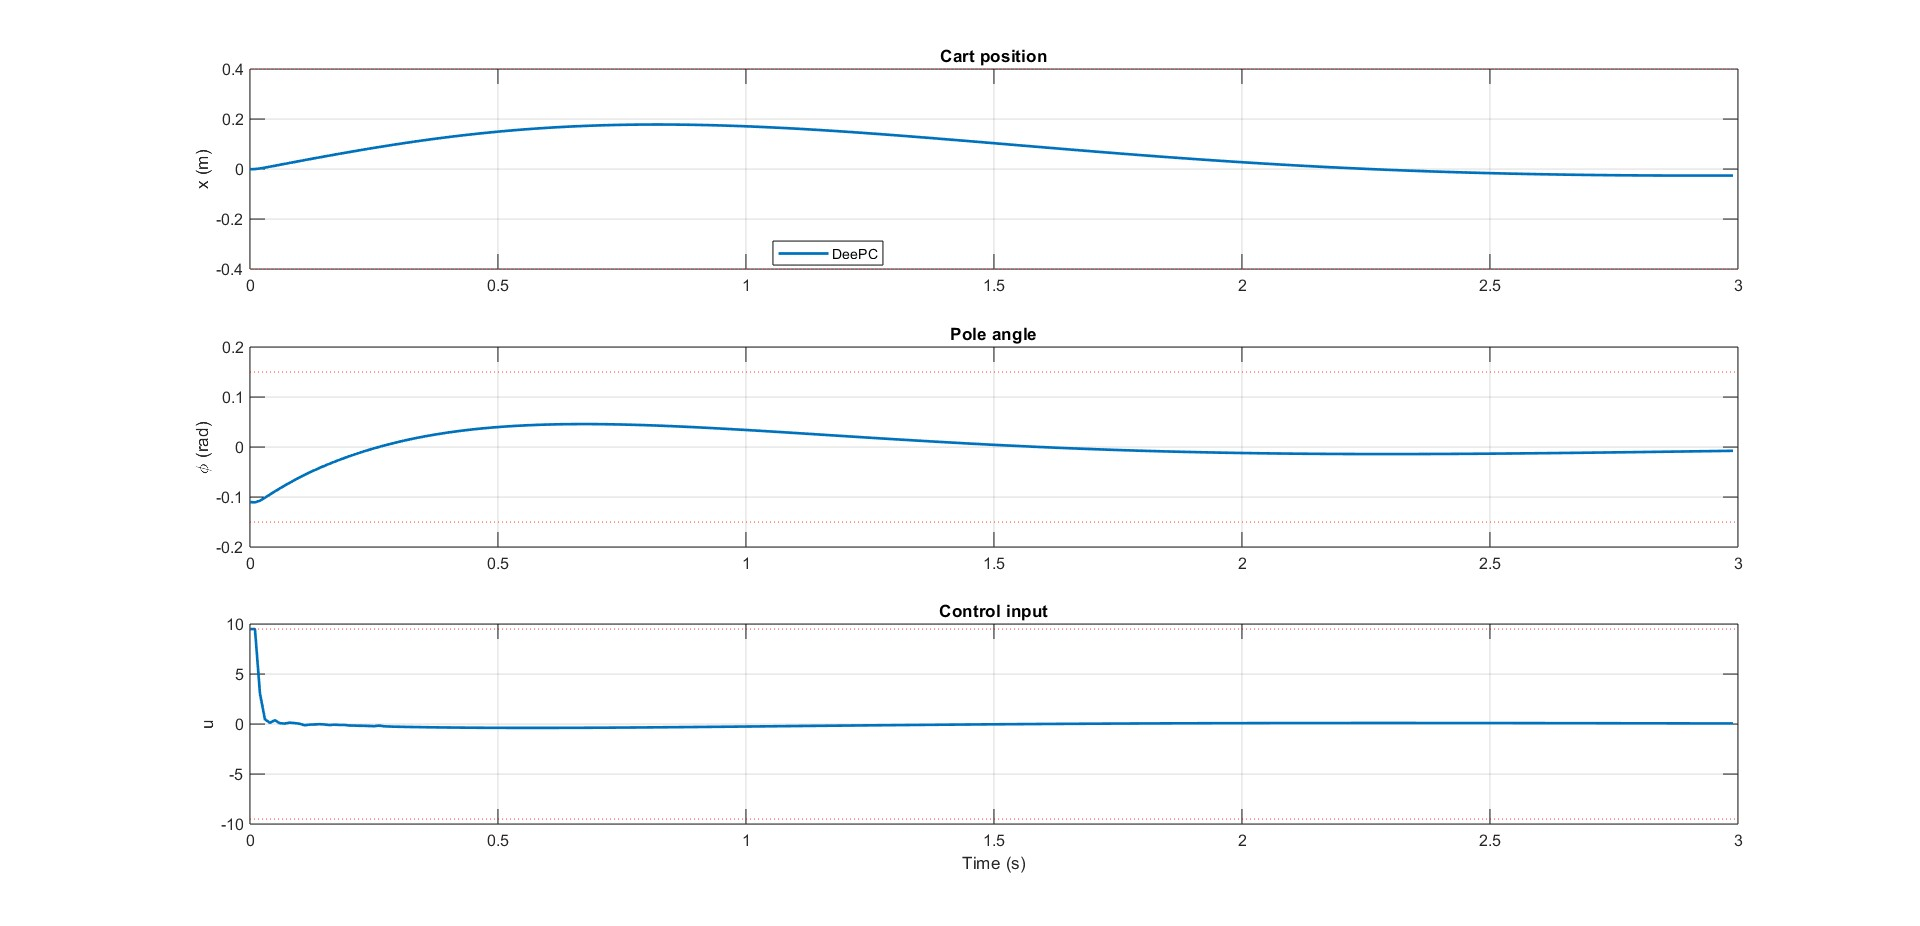
\includegraphics[width=0.88\linewidth]{first_traj_output.jpg}
        \caption{Closed-loop DeePC trajectory and input response.}
    \end{figure}
\end{frame}

\begin{frame}{State Trajectory}
    \begin{figure}
        \centering
        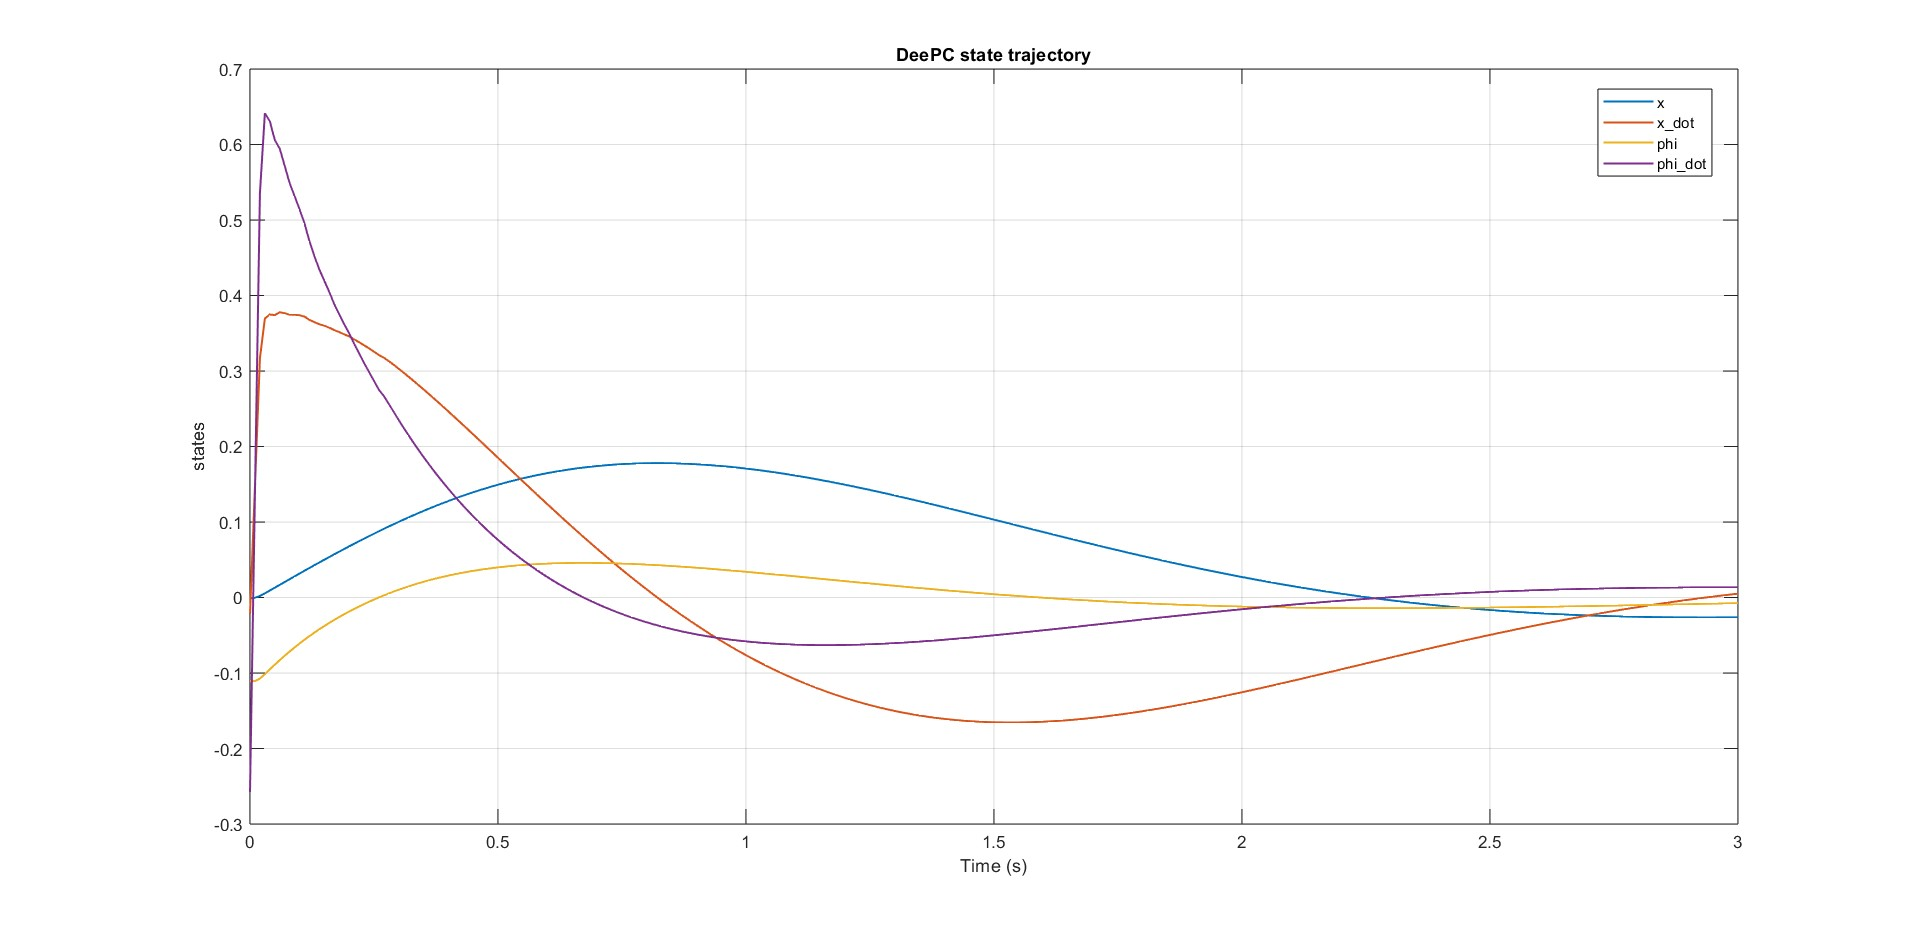
\includegraphics[width=0.88\linewidth]{first_all_state_output.jpg}
        \caption{Full state trajectory: cart position, cart velocity, pole angle, and pole angular velocity.}
    \end{figure}
\end{frame}

\begin{frame}{Regularization Diagnostics}
    \begin{figure}
        \centering
        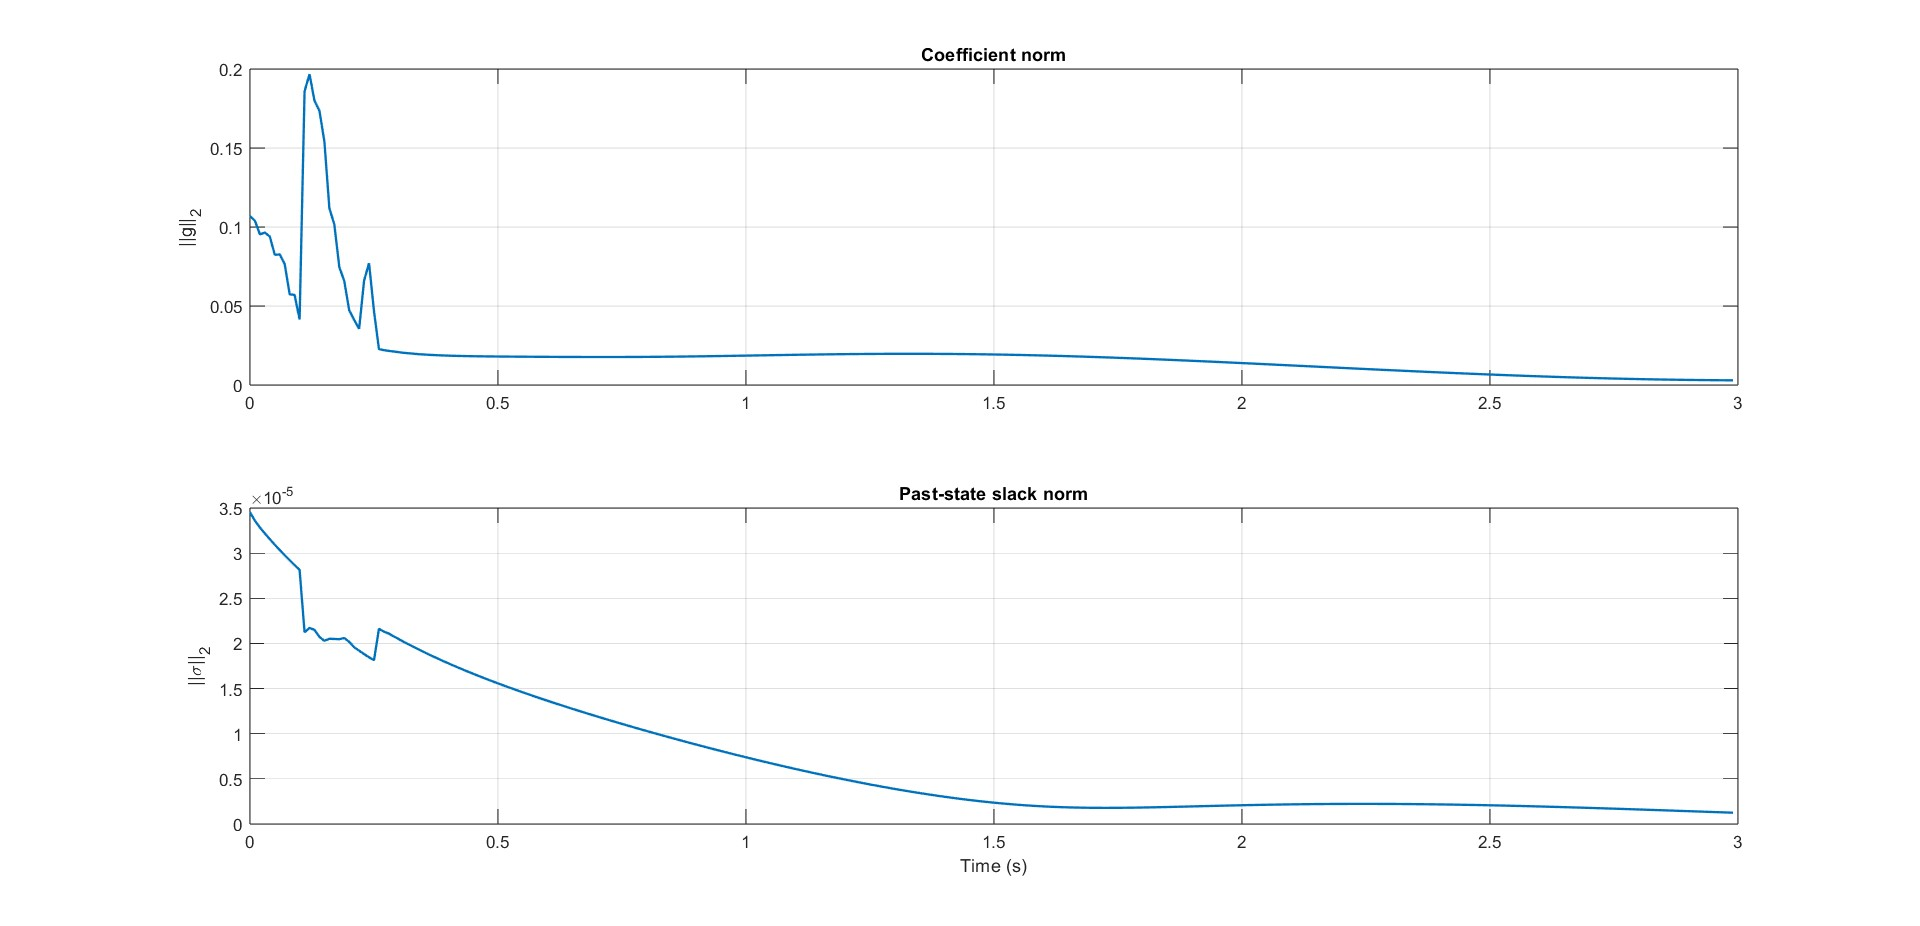
\includegraphics[width=0.88\linewidth]{first_norm_output.jpg}
        \caption{Norms of DeePC internal variables $g$ and $\sigma$.}
    \end{figure}
\end{frame}

\begin{frame}{Computation Time}
    \begin{figure}
        \centering
        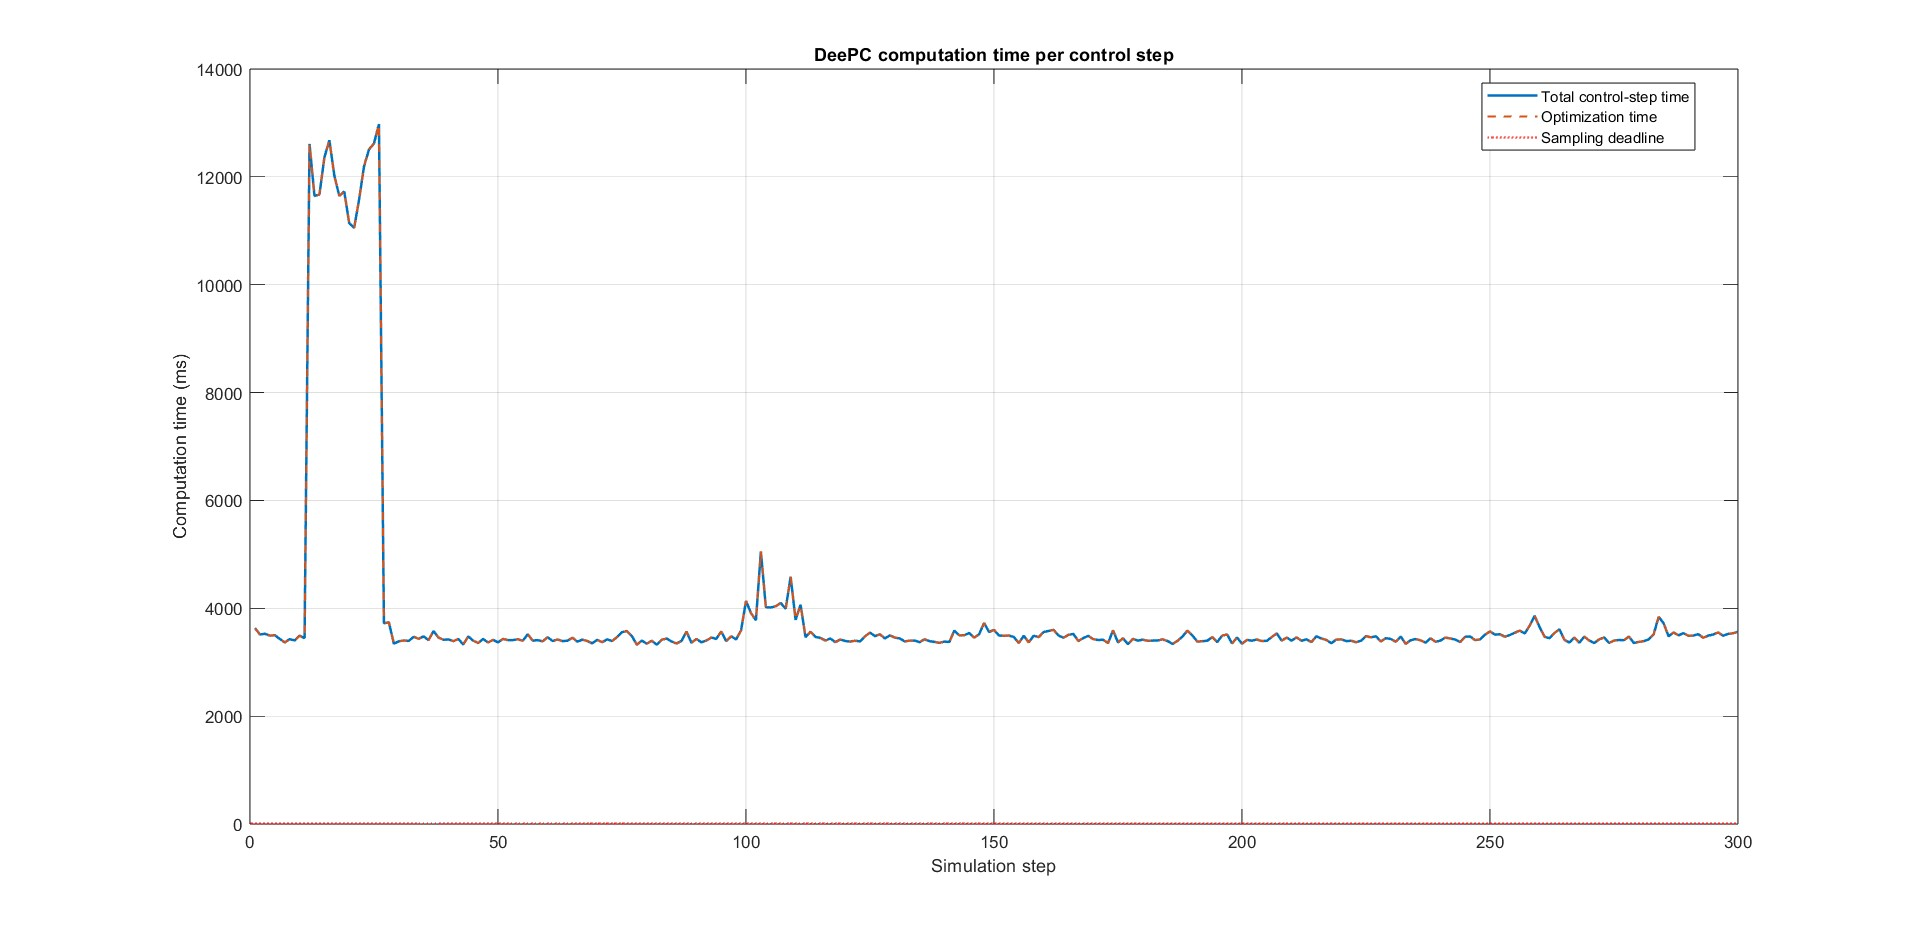
\includegraphics[width=0.88\linewidth]{first_compt_time_output.jpg}
        \caption{Optimization time and total control-step time compared with the sampling deadline.}
    \end{figure}
\end{frame}

\begin{frame}{Controller Comparison}
    \begin{table}
        \centering
        \small
        \begin{tabular}{p{2.4cm}p{4.0cm}p{4.0cm}}
            \toprule
            Method & Strengths & Limitations \\
            \midrule
            LQR
            & Very fast online control; simple stabilizing baseline.
            & No direct input or state constraints. \\
            \addlinespace
            Recursive MPC
            & Explicit model, input constraints, terminal target.
            & Requires reliable model; terminal equality can cause infeasibility. \\
            \addlinespace
            Regularized DeePC
            & Uses measured trajectories directly; includes constraints and robustness slack.
            & Requires rich data; larger QP due to Hankel coefficient vector $g$. \\
            \bottomrule
        \end{tabular}
    \end{table}
\end{frame}

\begin{frame}{Main Technical Findings}
    \begin{itemize}
        \item The linearized cart-pole requires careful handling because the upright equilibrium is unstable.
        \item LQR is useful both as a baseline controller and as a stabilizer during data collection.
        \item Recursive MPC gives a clear constrained model-based benchmark, but horizon length is critical.
        \item DeePC can produce predictive control behavior from data using Hankel matrices rather than an explicit prediction model.
        \item Regularization and slack are important for numerical robustness and noisy data consistency.
        \item Timing diagnostics are essential because the sampling time is only $10$ ms.
    \end{itemize}
\end{frame}

\begin{frame}{Limitations}
    \begin{itemize}
        \item The plant used for simulation is still the linearized model.
        \item DeePC performance depends strongly on data quality, excitation richness, and conditioning of the Hankel matrix.
        \item The current DeePC formulation uses full-state Hankel matrices, which assumes state availability.
        \item The terminal pole-angle equality improves regulation but may reduce feasibility.
        \item A fully fair comparison requires identical initial conditions, references, constraints, and cost definitions across LQR, MPC, and DeePC.
    \end{itemize}
\end{frame}

\begin{frame}{Future Work}
    \begin{itemize}
        \item Compare all controllers under identical initial conditions and references.
        \item Add quantitative metrics:
        \[
        \text{settling time},\quad
        \text{peak angle},\quad
        \text{control energy},\quad
        \text{constraint violations}.
        \]
        \item Test DeePC on noisy output-only measurements.
        \item Extend toward robust/kernelized DeePC for nonlinear behavior.
        \item Validate on the nonlinear cart-pole model rather than only the linearized dynamics.
    \end{itemize}
\end{frame}

\begin{frame}{Reviewer Takeaway}
    \begin{block}{Core message}
        This project builds a systematic path from model-based optimal control to data-enabled predictive control for the inverted pendulum.
    \end{block}

    \vspace{0.4cm}
    \begin{itemize}
        \item LQR provides the stabilizing reference point.
        \item MPC introduces constraints and receding-horizon optimization.
        \item DeePC replaces the explicit prediction model with measured trajectory data.
        \item Regularization, slack variables, and real-time diagnostics make the DeePC implementation more practical.
    \end{itemize}
\end{frame}

\begin{frame}
    \centering
    \Huge Questions?
\end{frame}

\end{document}
